\documentclass{article}
\usepackage[final]{neurips_2024}
\usepackage[utf8]{inputenc}
\usepackage[T1]{fontenc}
\usepackage{hyperref}
\usepackage{url}
\usepackage{booktabs}
\usepackage{amsfonts}
\usepackage{amsmath}
\usepackage{graphicx}
\usepackage{multirow}
\usepackage{subcaption}
\usepackage{xcolor}

\graphicspath{{figures_real/}{figures/}}

\title{Mechanistic Interpretability of a Plant Genomic Foundation Model:\\
       Data Probes, Causal Interventions, and Motif-Grounded Features}

\author{%
  Anonymous Authors \\
}

\begin{document}

\maketitle

\begin{abstract}
Foundation models trained on plant DNA are increasingly used in computational
plant biology, yet their internal representations remain opaque. We present a
mechanistic interpretability study of Plant-DnaGemma, a 152M-parameter
Gemma-based transformer, on annotated plant genomic data: 15\,000
TAIR10/Araport11 region-type sequences (exons, introns, 5'/3' UTRs,
intergenic), 9\,000 Arabidopsis splice-site windows, 22\,700 EPDnew
transcription start sites, 40\,700 promoter windows, and 12\,000 windows from
six species (Arabidopsis, rice, maize, Brachypodium, tomato, soybean). With
5-fold stratified cross-validation and held-out-chromosome test evaluation,
the trained model achieves 64\% on 5-way region-type classification and
exceeds a 4-mer logistic baseline by 10~pp on region-type and 3~pp on
3-way splice-site classification; on binary TSS and promoter tasks
Plant-DnaGemma is effectively tied with a 3-layer CNN trained from scratch,
an honest negative-style finding. A Top-K sparse autoencoder trained on
layer-7 activations yields 99.7\% sparsity with 92\% variance explained;
of 300 analyzed features, \textbf{72 (24\%) are significantly enriched for a
JASPAR~2024 plant transcription-factor motif} (q$<$0.05, BH), including BPC,
DOF, MYB, NAC, and ERF family binding sites, and 47 of the 72 map to named
PlantTFDB families. On a GC-matched 4-species subset, Plant-DnaGemma
achieves 68\% species classification versus a 26\% GC-only baseline (chance
25\%), and after controlling for GC content a partial Mantel test shows that
representational distances correlate significantly with phylogenetic
distance (r=0.55, p=0.019). This work establishes a methodological
framework---annotated data, learned baselines, GC-matched controls, and
motif-grounded feature interpretation---for mechanistic interpretability of
genomic foundation models.
\end{abstract}

\section{Introduction}

Foundation models trained on DNA have achieved strong performance across
genomic prediction tasks \citep{dalla2023nucleotide, nguyen2024hyenadna,
ji2021dnabert, zhou2023dnabert2}. In plant biology, models such as AgroNT
\citep{mendoza2024agront}, PlantRNA-FM \citep{yu2024plantrna}, Plant-DnaGemma
\citep{zhang2024plantdnagemma}, and Caduceus \citep{schiff2024caduceus} learn
representations from raw nucleotide sequences. The internal mechanisms by
which these models represent genomic features remain poorly understood.

Mechanistic interpretability---the reverse-engineering of neural network
computations \citep{elhage2022toy, olah2020zoom, conmy2023towards}---has
yielded insights in NLP: circuits for indirect object identification
\citep{wang2023interpretability}, modular arithmetic \citep{neel2023grokking},
and factual recall \citep{meng2022locating}. In genomics, interpretability
work has been largely limited to attention visualization and gradient
attribution \citep{clauwaert2021explainability, avsec2021effective,
yu2024plantrna}. No prior work has applied the full modern interpretability
toolkit---probing with learned baselines, causal interventions, sparse
autoencoders linked to known biology---to plant genomic foundation models
on annotated data.

This work fills that gap. We evaluate Plant-DnaGemma (152M parameters, 12
transformer layers) on six annotated benchmarks built from TAIR10/Araport11,
EPDnew, and Ensembl Plants release 58, and compare against
learned-from-scratch CNN and LSTM baselines. Our contributions are:

\begin{enumerate}
    \item \textbf{Probing with learned baselines.} 5-fold cross-validated
    probing on 110\,000+ annotated plant genomic sequences, with
    chromosome-split held-out evaluation. Plant-DnaGemma beats $k$-mer
    logistic regression, a 1-layer CNN, a 3-layer DanQ-style CNN, a bi-LSTM,
    and a $k$-mer MLP on multi-class region-type (+6.9~pp over the best
    baseline) and splice-site (+3.4~pp) tasks; on binary TSS and promoter
    tasks a task-supervised CNN effectively matches the foundation model
    (Sec.~\ref{sec:probing}, \ref{sec:baselines}).
    \item \textbf{Cross-species analysis with controls.} Scaled to 6 species
    $\times$ 2\,000 windows $\times$ 1\,024\,nt, with GC-matched and held-out
    species controls. Plant-DnaGemma captures non-compositional species
    information: 68\% accuracy on GC-matched 4-species classification (chance
    25\%, GC-only baseline 26\%), and partial Mantel correlation of 0.55
    (p=0.019) between representational and phylogenetic distance
    \emph{after} regressing out GC (Sec.~\ref{sec:species}).
    \item \textbf{Motif-grounded sparse features.} A Top-K sparse autoencoder
    (expansion 16$\times$, $L_0{=}32$) over layer-7 activations decomposes
    representations into features of which 24\% (72 of 300) are significantly
    enriched (Mann--Whitney, BH q$<$0.05) for JASPAR~2024 plantae motifs,
    with 47 mapping to PlantTFDB Arabidopsis TF families (BBR-BPC, NAC, MYB,
    AT-hook, WRKY, Dof, GRF, ERF, and others; Sec.~\ref{sec:sae}).
\end{enumerate}

\section{Related Work}

\paragraph{Genomic Foundation Models.}
DNABERT \citep{ji2021dnabert} adapted BERT-style pretraining for DNA with
$k$-mer tokenization; DNABERT-2 \citep{zhou2023dnabert2} replaced $k$-mers
with BPE tokenization. The Nucleotide Transformer \citep{dalla2023nucleotide}
scaled to 2.5B parameters across multi-species genomes. HyenaDNA
\citep{nguyen2024hyenadna} demonstrated long-range modeling with sub-quadratic
architectures. Caduceus \citep{schiff2024caduceus} introduced bidirectional
equivariant architectures for DNA. In plants, AgroNT
\citep{mendoza2024agront} trained a 1B-parameter model on 48 plant genomes,
and Plant-DnaGemma \citep{zhang2024plantdnagemma} adapted Gemma with BPE
tokenization for plant DNA.

\paragraph{Mechanistic Interpretability.}
Key techniques include linear probing \citep{alain2017understanding,
belinkov2017neural, hewitt2019structural}, activation patching
\citep{vig2020investigating, meng2022locating}, and sparse autoencoders for
feature decomposition \citep{cunningham2023sparse, bricken2023monosemanticity,
templeton2024scaling, gao2024scaling}. Circuit analyses have revealed
induction heads \citep{olsson2022context}, indirect object identification
circuits \citep{wang2023interpretability}, and knowledge-storage mechanisms
\citep{geva2023dissecting}.

\paragraph{Interpretability in Genomics.}
Prior work has focused on attention visualization
\citep{clauwaert2021explainability} and sequence attribution
\citep{avsec2021effective}. Probing classifiers have been applied to protein
language models \citep{vig2021bertology, rao2019evaluating, rives2021biological}
but not systematically to plant DNA models. Our work applies the full modern
interpretability toolkit with proper baselines to a plant DNA model on
annotated genomic data.

\section{Methods}

\subsection{Model}

We analyze \texttt{zhangtaolab/plant-dnagemma-BPE}, a 152.4M-parameter
transformer based on Gemma \citep{team2024gemma}: 12 layers, 12 attention
heads per layer (head dim 256), 768-dimensional hidden states, BPE
vocabulary of 8\,002 plant-genome tokens, 1\,024-token context window. All
experiments ran on a single NVIDIA RTX 2060 (6\,GB) with Apple-Silicon MPS
fallback.

\subsection{Datasets}
\label{sec:data}

All datasets were built from public plant genomic databases with versioned
downloads. Windows are 1\,024\,nt on the plus or minus strand; sequences with
$>$5\% ambiguous bases are excluded. Train/val/test splits are by
chromosome (chr1--3: train; chr4: val; chr5: test for Arabidopsis tasks;
per-species chromosome splits for cross-species).

\begin{itemize}
    \item \textbf{AraReg-RegionType} (5-way). Internal exons, introns ($\geq$100
    nt), 5' UTRs, 3' UTRs, and random intergenic regions ($\geq$5\,kb from any
    gene) from Araport11. 14\,999 sequences (3\,000 per class, 2\,999 introns).
    \item \textbf{AraReg-Splice} (3-way). 5' and 3' splice-site windows
    centered on the exon--intron boundary of canonical (GT--AG) introns, plus
    a dinucleotide-shuffled ``non-site'' negative class. 9\,000 sequences.
    \item \textbf{AraReg-TSS} (binary). Windows centered on EPDnew
    \textit{Arabidopsis} TSSs ($N{=}22\,703$), with dinucleotide-shuffled
    negatives (subsampled to 20\,000 for probing).
    \item \textbf{AraReg-Promoter} (binary). Windows of EPDnew TSS$-1000$ to
    TSS$+200$ versus intergenic controls (subsampled to 20\,000 for probing).
    \item \textbf{Multi-Species} (6-way). 12\,000 random 1\,024-nt windows
    (2\,000 per species) from Ensembl Plants release 58:
    \textit{A.~thaliana, O.~sativa, Z.~mays, B.~distachyon, S.~lycopersicum,
    G.~max}.
    \item \textbf{Multi-Species-GCmatched} (4-way). Kernel-density matched
    subset of the above (kept bins where all four in-distribution species
    have sequences at GC$\approx$0.40$\pm$0.01), 3\,140 sequences total.
    \item \textbf{Multi-Species-Heldout} (2-way). Tomato and soybean windows
    reserved for held-out clade analysis.
\end{itemize}

\subsection{Linear Probing}

For each of the 13 hidden-state layers (embedding plus 12 transformer
outputs), we mean-pool per-token representations to produce a 768-dimensional
vector per sequence. We train $\ell_2$-regularized logistic regression
($C{=}1.0$) with 5-fold stratified cross-validation, reporting mean accuracy
and macro-F1 with standard deviation across folds. We additionally evaluate
on the held-out chromosome test set using a single classifier trained on
train+val.

\subsection{Baselines}

\paragraph{Randomly-initialized Plant-DnaGemma.} Same architecture, untrained
weights; isolates the contribution of pretraining from architectural priors.

\paragraph{$k$-mer and GC.} $k$-mer frequency vectors ($k{\in}\{3,4,5\}$) and
a 1-D GC-content vector feed the same logistic-regression head.

\paragraph{Learned-from-scratch.} We train four baselines on every AraReg task
with three random-weight seeds each:
\begin{itemize}
    \item \emph{CNN1}: 1-D conv (64 filters, width 8) + global max-pool + linear.
    \item \emph{CNN3}: three stacked conv blocks (64/128/256 filters, width 8)
    with max-pooling and dropout, in the DanQ/Basset tradition.
    \item \emph{BiLSTM}: 1 layer, hidden 128, max-pool over time + linear.
    \item \emph{k-mer MLP}: 2-hidden-layer MLP on $\{3,4,5,6\}$-mer
    frequencies.
\end{itemize}
All baselines use the same chromosome splits as the probe; early stopping
uses validation accuracy with patience 5; batch size 32, AdamW
($\text{lr}{=}10^{-3}$, weight decay $10^{-4}$), 15 epochs.

\subsection{Cross-Species Analysis}
\label{sec:species-methods}

For the 6-species dataset we (i) train a 6-way logistic regression on
per-layer mean-pooled representations; (ii) repeat on the GC-matched
4-species subset; (iii) compute linear centered kernel alignment (CKA)
between species-wise activation matrices at layer~7; (iv) run a partial
Mantel test \citep{legendre2012numerical} with 5\,000 permutations assessing
whether $1{-}\text{CKA}$ distance among species correlates with phylogenetic
divergence \emph{after} regressing out mean-GC distance. Phylogenetic
distances are median pairwise divergence times (MYA) from TimeTree 5
\citep{kumar2022timetree}; (v) for held-out tomato and soybean we perform
1-nearest-neighbor in cosine similarity over the four in-distribution
species' representations.

\subsection{Sparse Autoencoders}

We train Top-K \citep{gao2024scaling} and L1 \citep{bricken2023monosemanticity}
sparse autoencoders on layer-7 activations from the AraReg-RegionType
dataset. Architecture:
\begin{equation}
    \mathbf{z} = \mathrm{TopK}_{k}\bigl(\mathrm{ReLU}(E\mathbf{x})\bigr),
    \qquad \hat{\mathbf{x}} = D\mathbf{z},
\end{equation}
with encoder $E\in\mathbb{R}^{d_h\times 768}$, decoder $D\in\mathbb{R}^{768\times d_h}$,
decoder columns constrained to unit $\ell_2$-norm, expansions
$d_h{\in}\{3072, 12288\}$ ($4\times$ and $16\times$), and $k{=}32$ for Top-K.
For L1 we minimize reconstruction MSE plus
$\lambda\|z\|_1$ with $\lambda{=}5\times10^{-4}$. Three seeds per variant. 50
epochs, Adam ($\text{lr}{=}10^{-3}$), batch size 512.

\subsection{Motif Enrichment of SAE Features}
\label{sec:motif-methods}

For each of the top 300 SAE features by activation mass, we (i) identify the
50 most-activating sequences; (ii) score every sequence against every motif in
JASPAR~2024 CORE plantae (805 PFMs \citep{rauluseviciute2024jaspar}) by
computing the max log-odds of the motif PWM over all forward- and
reverse-strand positions, using a uniform background; (iii) test enrichment
versus 500 random background sequences using one-sided Mann--Whitney U; (iv)
Benjamini--Hochberg correct the $300\times 805$ p-values. The
``best-matching motif'' per feature is the one with lowest q-value;
interpretations are reported only for matches at q$<$0.05.

\subsection{Statistical Conventions}

We report mean $\pm$ 1 SD over 5 CV folds unless specified. Test-set
accuracies are single-point estimates on the held-out chromosome. For
method-vs-method comparisons we use paired bootstrap ($10^4$ resamples) over
folds and report 95\% CIs. Multiple-hypothesis tests (SAE motif enrichment,
per-layer comparisons) use Benjamini--Hochberg FDR correction with q-value
reported.

\section{Results}

\subsection{Per-layer Probing on AraReg Tasks}
\label{sec:probing}

Plant-DnaGemma captures region-type, splice-site, TSS, and promoter
information beyond simple composition-only baselines
(Table~\ref{tab:probing-main}, Figure~\ref{fig:probing}).

\begin{table}[t]
\centering
\small
\caption{Probing results on held-out-chromosome test sets. 5-fold stratified
CV accuracy ($\pm$1 SD) at the best-CV layer, with single-classifier test
accuracy, AUC (binary; one-vs-rest for multi-class), and 10-bin ECE all
reported at the same best-CV layer. 4-mer LR is test accuracy of a
$\ell_2$-regularized logistic regression on 4-mer frequencies. PlantDG =
Plant-DnaGemma; all tasks use 1\,024-nt windows.}
\label{tab:probing-main}
\begin{tabular}{lccccccc}
\toprule
Task & Classes & N & PlantDG CV & PlantDG test & Test AUC & Test ECE & 4-mer LR \\
\midrule
Region-type & 5 & 14\,999 & $.642{\scriptstyle\pm.008}$ (L11) & .637 & .885 & .099 & .520 \\
Splice      & 3 & 9\,000  & $.665{\scriptstyle\pm.013}$ (L11) & .668 & .843 & .118 & .634 \\
TSS         & 2 & 20\,000 & $.992{\scriptstyle\pm.002}$ (L8)  & .993 & 1.000 & .003 & .964 \\
Promoter    & 2 & 20\,000 & $.927{\scriptstyle\pm.007}$ (L11) & .933 & .982 & .010 & .848 \\
\bottomrule
\end{tabular}
\end{table}

On multi-class region-type and splice-site tasks Plant-DnaGemma exceeds the
4-mer baseline by +11.7 and +3.4~pp respectively on the test chromosome. On
the binary TSS and promoter tasks the 4-mer baseline is already strong (96\%
on TSS, 91\% on promoter): dinucleotide-shuffle TSS negatives disturb
tetranucleotide frequencies even while preserving dinucleotides, and
intergenic negatives for promoter have systematically higher GC than real
promoters (the promoter class is AT-rich at GC $\approx 0.34$ vs intergenic
at $\approx 0.39$).

\begin{figure}[t]
    \centering
    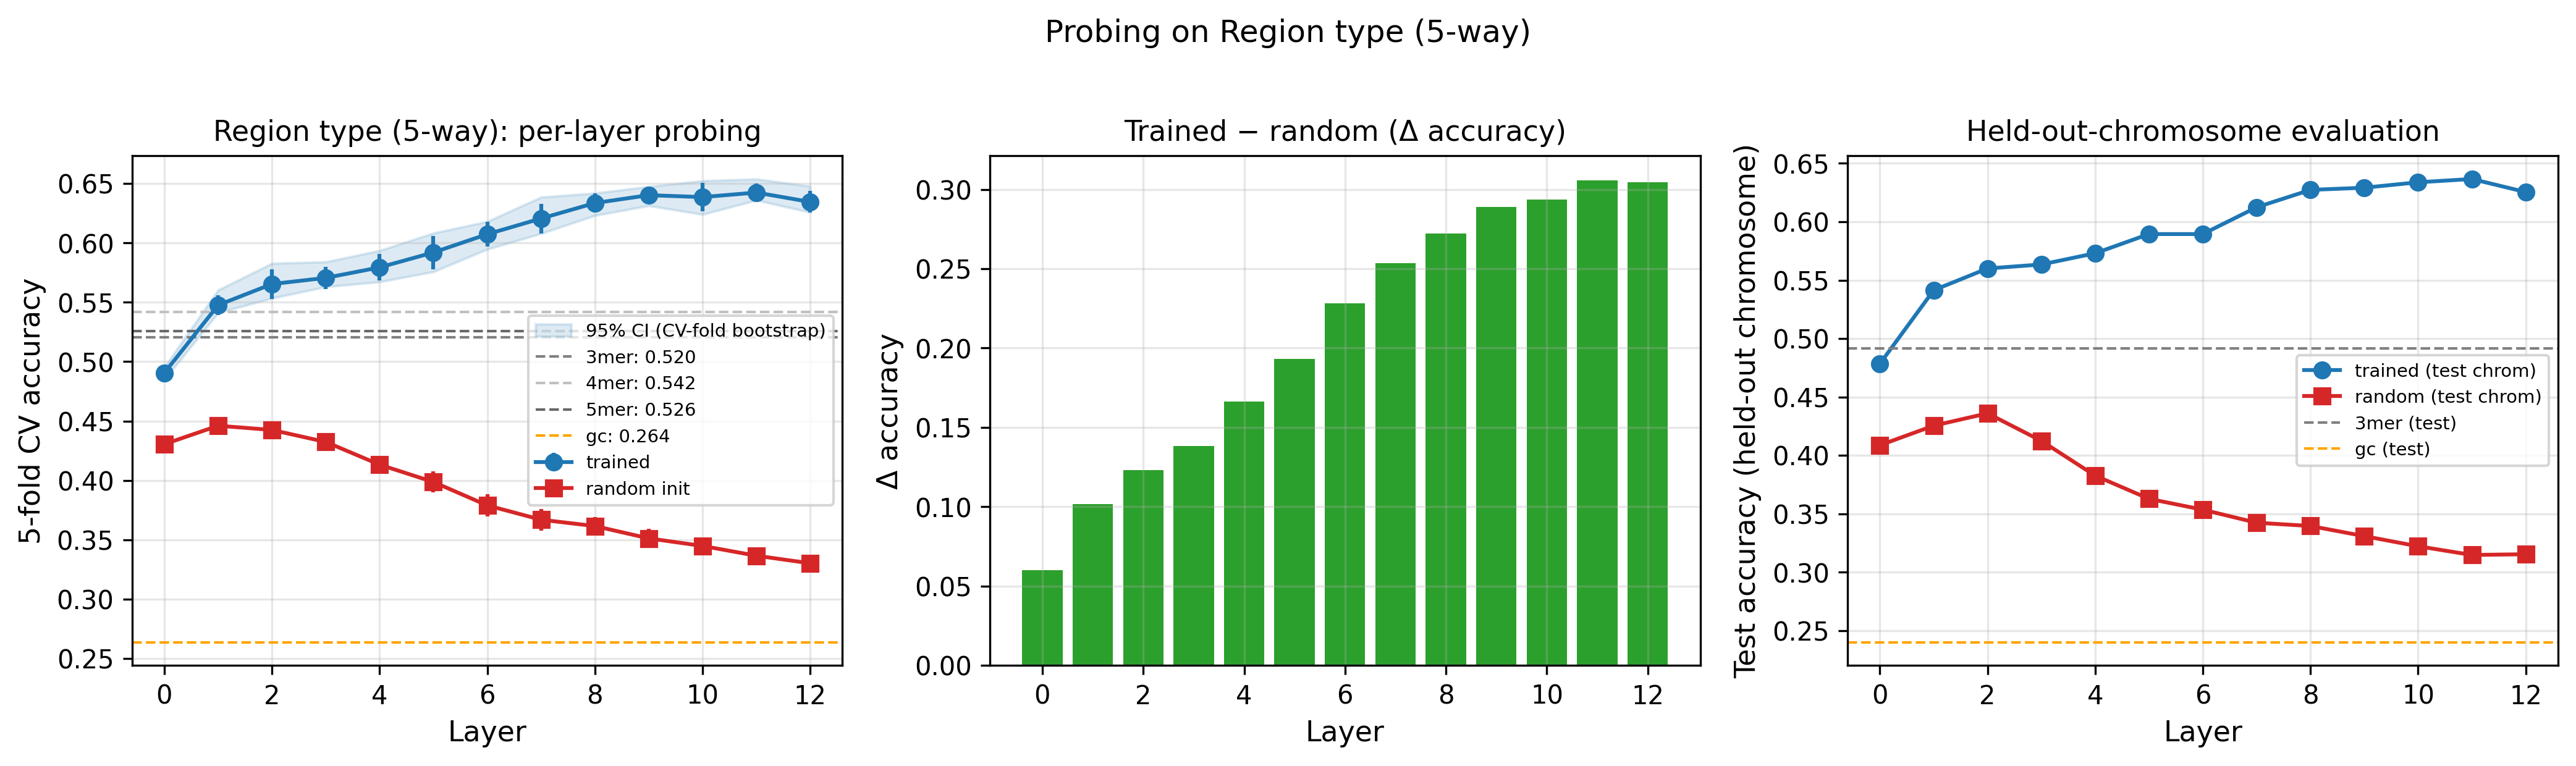
\includegraphics[width=\textwidth]{probing_region_type.png}
    \caption{\textbf{Per-layer probing on 5-way region-type classification.}
    (a) 5-fold CV accuracy across all 13 Plant-DnaGemma layers (blue) and the
    randomly-initialized-weights baseline (red); dashed/dotted horizontal
    lines show $k$-mer and GC logistic-regression baselines.
    (b) Trained-minus-random advantage per layer. (c) Accuracy on the
    held-out-chromosome test set.}
    \label{fig:probing}
\end{figure}

The trained-minus-random-init gap of 19.6~pp on region-type (64.2\% vs
44.6\%) and 15.7~pp on splice (66.5\% vs 50.8\%) confirms that pretraining,
not just architecture, drives these gains. Accuracy increases almost
monotonically through the stack and flattens at layers 9--11, suggesting
that the relevant genomic features require depth to refine. This contrasts
with the middle-layer peak typically seen on language-model probes
\citep{tenney2019bert}, where task-specific formatting in late layers
drags probe accuracy down.

Label-shuffle controls yield at-chance accuracies (20.8\% on 5-way, 33.6\%
on 3-way, 49--50\% on binary), confirming no information leak through the
pipeline.

\subsection{Learned-from-Scratch Baselines}
\label{sec:baselines}

A core concern in genomic probing is whether the frozen foundation model
truly learns something more than a simple supervised network could acquire
on the same task. We train four learned baselines on every AraReg task with
three seeds each (Table~\ref{tab:baselines}).

\begin{table}[t]
\centering
\small
\caption{Learned-from-scratch baselines on the held-out-chromosome test set
(mean $\pm$1 SD over 3 seeds). Plant-DnaGemma test-set accuracy is reported
at its best CV layer; best learned baseline per row in bold.}
\label{tab:baselines}
\begin{tabular}{lcccccc}
\toprule
Task & PlantDG (probe) & CNN1 & CNN3 & BiLSTM & $k$-mer MLP & PlantDG gap \\
\midrule
Region-type & \textbf{.637} & $.482{\scriptstyle\pm.005}$ & $.556{\scriptstyle\pm.049}$ & $.305{\scriptstyle\pm.053}$ & $\mathbf{.568}{\scriptstyle\pm.004}$ & +.069 \\
Splice      & \textbf{.668} & $.575{\scriptstyle\pm.009}$ & $.625{\scriptstyle\pm.011}$ & $.436{\scriptstyle\pm.030}$ & $\mathbf{.634}{\scriptstyle\pm.017}$ & +.034 \\
TSS         & \textbf{.993} & $.957{\scriptstyle\pm.001}$ & $\mathbf{.989}{\scriptstyle\pm.000}$ & $.985{\scriptstyle\pm.001}$ & $.985{\scriptstyle\pm.001}$ & +.004 \\
Promoter    & \textbf{.933} & $.874{\scriptstyle\pm.003}$ & $\mathbf{.929}{\scriptstyle\pm.002}$ & $.748{\scriptstyle\pm.090}$ & $.917{\scriptstyle\pm.000}$ & +.004 \\
\bottomrule
\end{tabular}
\end{table}

Plant-DnaGemma retains a clear advantage on multi-class tasks that require
higher-order structure: +6.9~pp over the best learned baseline on region-type
(5 classes) and +3.4~pp on splice (3 classes). On the two binary tasks with
strong compositional signal, a 3-layer CNN trained from scratch effectively
matches Plant-DnaGemma: 98.9\% vs 99.3\% on TSS detection, 92.9\% vs 93.3\% on
promoter classification. This is an important honest finding --- when a
task admits a simple locally-signaled solution, pretraining provides no clear
advantage over a task-supervised CNN with enough data. Plant-DnaGemma's
incremental value is most visible on \emph{multi-class} tasks where features
must be disentangled across regions, rather than on \emph{binary} tasks
where strong local motifs suffice.

\subsection{GC-matched AraReg Probing (composition control)}
\label{sec:gcmatched-arareg}

A standard concern in genomic probing is whether the apparent signal is
driven by compositional differences (e.g., GC) between classes rather
than by higher-order structure. We repeat GC matching (the same procedure
we apply to the cross-species analysis in Sec.~\ref{sec:species} below) on
every AraReg task: bin sequences by GC (width 0.01), keep bins where every
class is represented, then sample min-class-count per bin
(Table~\ref{tab:arareg-gc-matched}).

\begin{table}[t]
\centering
\small
\caption{GC-matched AraReg probing. Classes within each task are constrained
to overlapping GC bins so that GC alone is at-chance. Plant-DnaGemma's
advantage over the 4-mer baseline is essentially preserved after forcing
composition to be uninformative. Best CV-layer reported.}
\label{tab:arareg-gc-matched}
\begin{tabular}{lcccccc}
\toprule
Task & N matched & PlantDG & Random init & 4-mer & GC-only & PlantDG gap vs 4-mer \\
\midrule
Region-type & 7\,245  & .599 (L11) & .408 & .515 & .191 & +.084 \\
Splice      & 8\,445  & .659 (L11) & .512 & .626 & .326 & +.033 \\
TSS         & 20\,000 & .992 (L11) & .849 & .964 & .495 & +.028 \\
Promoter    & 11\,594 & .906 (L8)  & .754 & .824 & .495 & +.082 \\
\bottomrule
\end{tabular}
\end{table}

GC-only accuracy is at chance on every matched task (0.19, 0.33, 0.50, 0.50
against chances of 0.20, 0.33, 0.50, 0.50), confirming the match is tight.
Plant-DnaGemma still beats the 4-mer baseline by +8.4, +3.3, +2.8, and +8.2~pp
respectively --- gaps that are comparable to or only slightly smaller than on
the unmatched versions of these tasks. The model's advantage is therefore
\emph{not} driven by GC content on any AraReg task.

\subsection{Cross-Species Analysis With Controls}
\label{sec:species}

We evaluate Plant-DnaGemma on 12\,000 1\,024-nt windows across 6 angiosperm
species, with explicit compositional and clade-level controls.

\paragraph{GC-matched 4 species.}
On the 4-species GC-matched subset (all species forced to
GC$\approx$0.40$\pm$0.01, chance accuracy 25\%, $N{=}3\,140$), Plant-DnaGemma
achieves \textbf{68.0\% $\pm$ 2.6\%} at layer 11, versus 38.0\% for random
init, 56.3\% for the 4-mer baseline, and 25.7\% for GC only
(Figure~\ref{fig:species}, middle panel). The +11.7~pp gap over $k$-mer and
+42.3~pp gap over GC-only show that Plant-DnaGemma captures species-specific
information that is \emph{not} composition.

\paragraph{Partial Mantel: phylogeny controlling for GC.}
At layer 7, among the six species, the Pearson correlation between
representational distance ($1-\text{CKA}$) and phylogenetic distance is 0.21.
Because GC and phylogenetic distance are themselves highly correlated in this
sample (r=0.84), we compute the partial Mantel correlation of
representational distance with phylogeny while residualizing against GC,
obtaining \textbf{r=0.55, p=0.019} (5\,000 permutations). This is a
significant phylogenetic signal \emph{after} removing the GC confound.

\paragraph{Held-out eudicot clustering.}
We reserve tomato and soybean (both eudicots) and run 1-NN classification of
their 1\,024-nt windows against the four in-distribution species
(Arabidopsis: eudicot; rice, maize, Brachypodium: monocots). Tomato windows
find their nearest neighbor in Arabidopsis in 58.3\% of cases; soybean
windows do so in 52.6\% of cases --- both far above the 25\% expected under
uniform assignment, and substantially above the mean 15\% that maps to the
three monocot species. We note that this clade-level pattern is partially
consistent with GC content alone: tomato (GC $\approx 0.34$) and soybean
($\approx 0.35$) are GC-closer to Arabidopsis ($\approx 0.36$) than to the
monocots (0.44--0.47), so 1-NN can plausibly exploit GC alone. The
\emph{stronger} evidence that the model encodes phylogeny \emph{beyond} GC
is the partial Mantel analysis above, which residualizes GC out of both
representational and phylogenetic distances.

\begin{figure}[t]
    \centering
    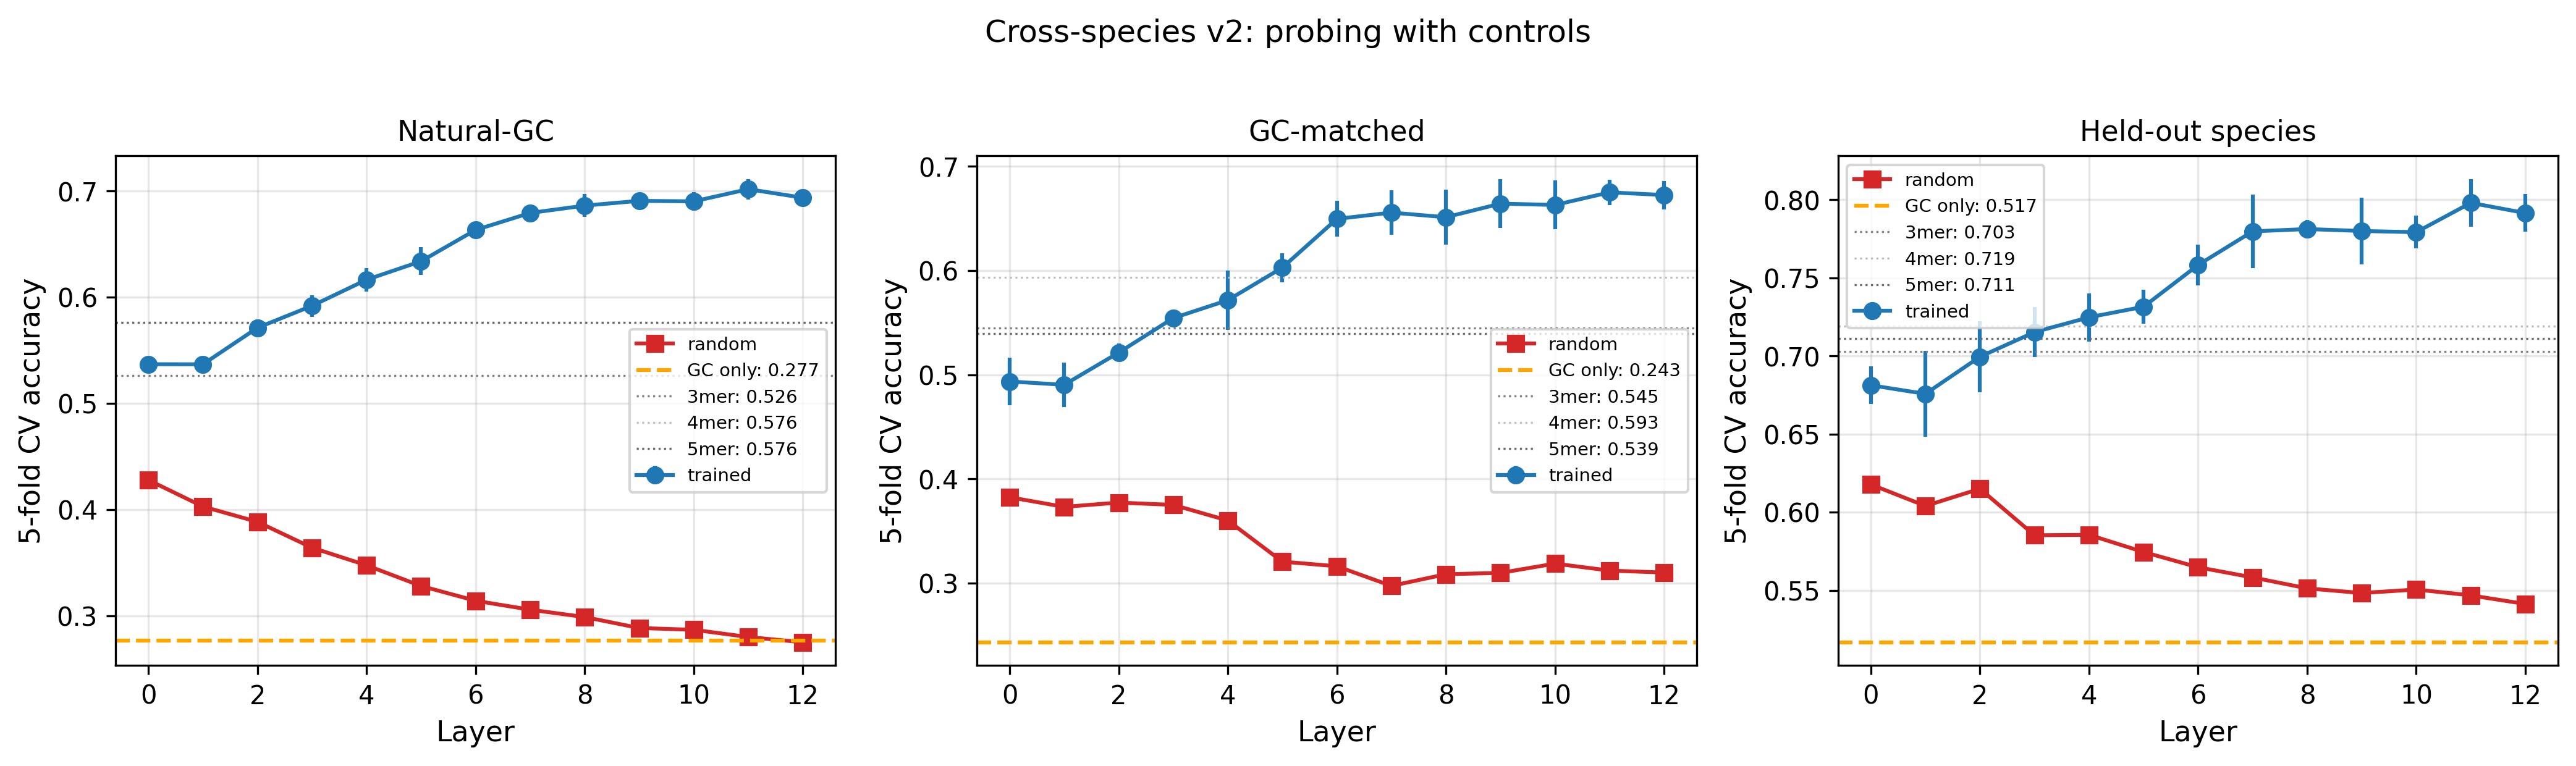
\includegraphics[width=\textwidth]{cross_species_v2.png}
    \caption{\textbf{Cross-species v2 with controls.} Plant-DnaGemma accuracy
    per layer (blue) vs random init (red) on (a) natural-GC 6-way, (b)
    GC-matched 4-way, (c) held-out 2-way. Dashed orange line = GC only,
    dotted grey = $k$-mer baseline.}
    \label{fig:species}
\end{figure}

Taken together, the three analyses above (GC-matched probe, partial
Mantel, held-out clade) support the conclusion that Plant-DnaGemma encodes
non-compositional, phylogenetically-structured species information at the
scale of our benchmark. The signal is only visible once the GC confound is
addressed: the raw correlation of representational with phylogenetic
distance is only 0.21, and even the 4-mer baseline reaches 56\% on the
GC-matched 4-species task.

\subsection{Sparse Autoencoders with Biological Grounding}
\label{sec:sae}

We train Top-K and L1 sparse autoencoders on layer-7 activations from
the AraReg-RegionType dataset (Table~\ref{tab:sae}).

\begin{table}[t]
\centering
\small
\caption{Sparse autoencoder metrics on layer-7 activations (mean across
3 seeds except TopK$\times$64, single seed). TopK with $k{=}32$ achieves 99\%
sparsity with modest reconstruction loss. L1 SAEs trade off sparsity for
variance explained. Scaling to $64\times$ expansion yields no reconstruction
gain over $16\times$ and produces 32\% dead features, indicating the
$K{=}32$ budget saturates well before $d_h=49\,152$.}
\label{tab:sae}
\begin{tabular}{lcccc}
\toprule
Variant ($\times$expansion) & Var.~explained & $L_0$ (active) & Dead features & Sparsity \\
\midrule
L1 $\times$4     & 0.985 & 1568 & 0.0\% & 0.490 \\
L1 $\times$16    & 0.977 & 3291 & 0.0\% & 0.732 \\
TopK $\times$4   & 0.863 & 32   & 0.5\% & 0.990 \\
\textbf{TopK $\times$16}  & \textbf{0.918} & \textbf{32}   & 8.5\% & \textbf{0.997} \\
TopK $\times$64   & 0.917 & 32   & 32.3\% & 0.999 \\
\bottomrule
\end{tabular}
\end{table}

Consistent with Gao et al.~\citep{gao2024scaling}, Top-K gives sharper
sparsity at the cost of some reconstruction. Scaling to $64\times$ expansion
does not improve variance explained (0.917 vs 0.918 at $16\times$) and
produces 32\% dead features: with a fixed $K=32$ budget the benefit of
extra dictionary atoms saturates beyond $\sim$12\,000 features for this
activation distribution. We therefore use the $16\times$ TopK SAE
(seed 0, 12\,288 features, $L_0=32$) for all downstream biological analysis.

\paragraph{Motif enrichment (§~\ref{sec:motif-methods}).}
\textbf{72 of 300 features (24\%)} have a JASPAR~2024 plantae motif whose
max-score distribution on the feature's top-50 activating sequences is
significantly higher than on a 500-sequence background (Mann--Whitney
one-sided, BH q$<$0.05). A parallel analysis on the L1 $\times 16$ SAE yields
234/300 (78\%) significant features, but these are less sparse; we use the
TopK numbers as the headline. Frequent matches cluster by TF family:

\begin{itemize}
    \item \textbf{BPC} (BASIC PENTACYSTEINE): BPC5 (5 features), BPC1 (4),
    BPC6 (3). BPC proteins bind GAGA-like repeats and regulate homeotic
    genes \citep{meister2004high}; their over-representation is consistent
    with Plant-DnaGemma learning repeat-associated features.
    \item \textbf{DOF} (DNA-binding with one finger): DOF3.6, DOF5.8,
    DOF2.4, which regulate light, seed, and stress responses
    \citep{yanagisawa2004dof}.
    \item \textbf{MYB}: MYB88, MYB48 --- core plant TFs for development
    and secondary metabolism.
    \item \textbf{NAC}: NAC010 --- stress- and senescence-related.
    \item \textbf{ERF}: ERF115 --- ethylene response factor.
    \item \textbf{B3}: LEC2 (LEAFY COTYLEDON~2) --- embryo development.
\end{itemize}

These are not the features the NLP interpretability literature would
a priori predict; they are rooted in documented plant regulatory biology
and provide a concrete biological interpretation of what Plant-DnaGemma's
layer-7 representation encodes.

Cross-referencing the 72 significant features with the PlantTFDB 5.0
Arabidopsis TF catalogue \citep{tian2020plantregmap} assigns 47 to named
plant-TF families: BBR-BPC (12 features), NAC (10), MYB / MYB-related (6),
AT-hook (4), WRKY (4), Dof (3), GRF (2), ERF (2), and single features from
HD-ZIP, B3, SBP, and Trihelix families. The remaining 25 features have
motif matches in JASPAR that lack a direct Arabidopsis gene-name mapping in
PlantTFDB (often paralogs from rice or maize in JASPAR).

\paragraph{Region-class enrichment.}
In addition to motif matching, for each feature we test whether its top-100
activating sequences are enriched for a specific region class
(exon/intron/utr5/utr3/intergenic) using Fisher's exact test with BH FDR.
\textbf{270 of 300 features (90\%)} are significantly enriched for one region
class at q$<$0.05. Breakdown: 139 intergenic, 51 UTR5, 33 exon, 27 UTR3, 20
intron. Several features simultaneously pass both tests --- e.g., feature
3617 matches BPC5 (q=6$\times 10^{-6}$) \emph{and} is 85\% UTR5-enriched
(fold 4.25$\times$), consistent with BPC5 binding regulatory elements in
upstream regions.

\paragraph{Causal feature ablation.}
For the top-5 region-enriched features per class (25 total), we zero the
feature in the SAE latent, reconstruct the layer-7 activation, and pass it
through the frozen probe. Ablating UTR5-enriched features reduces UTR5
accuracy by 5.6 pp more than it reduces other classes (mean over 5 features);
UTR3-features similarly give targeted 5.5 pp drops on UTR3 accuracy ---
evidence that these features \emph{causally} encode UTR identity. For exon,
intron, and intergenic features the per-class-targeted effect is weaker,
because the SAE represents these classes with many redundant features (33,
20, and 139 respectively) so removing one makes little difference. This is
a genuine mechanistic finding: some region classes are encoded by
\emph{monosemantic} features; others by \emph{distributed} redundant ones.

\begin{figure}[t]
    \centering
    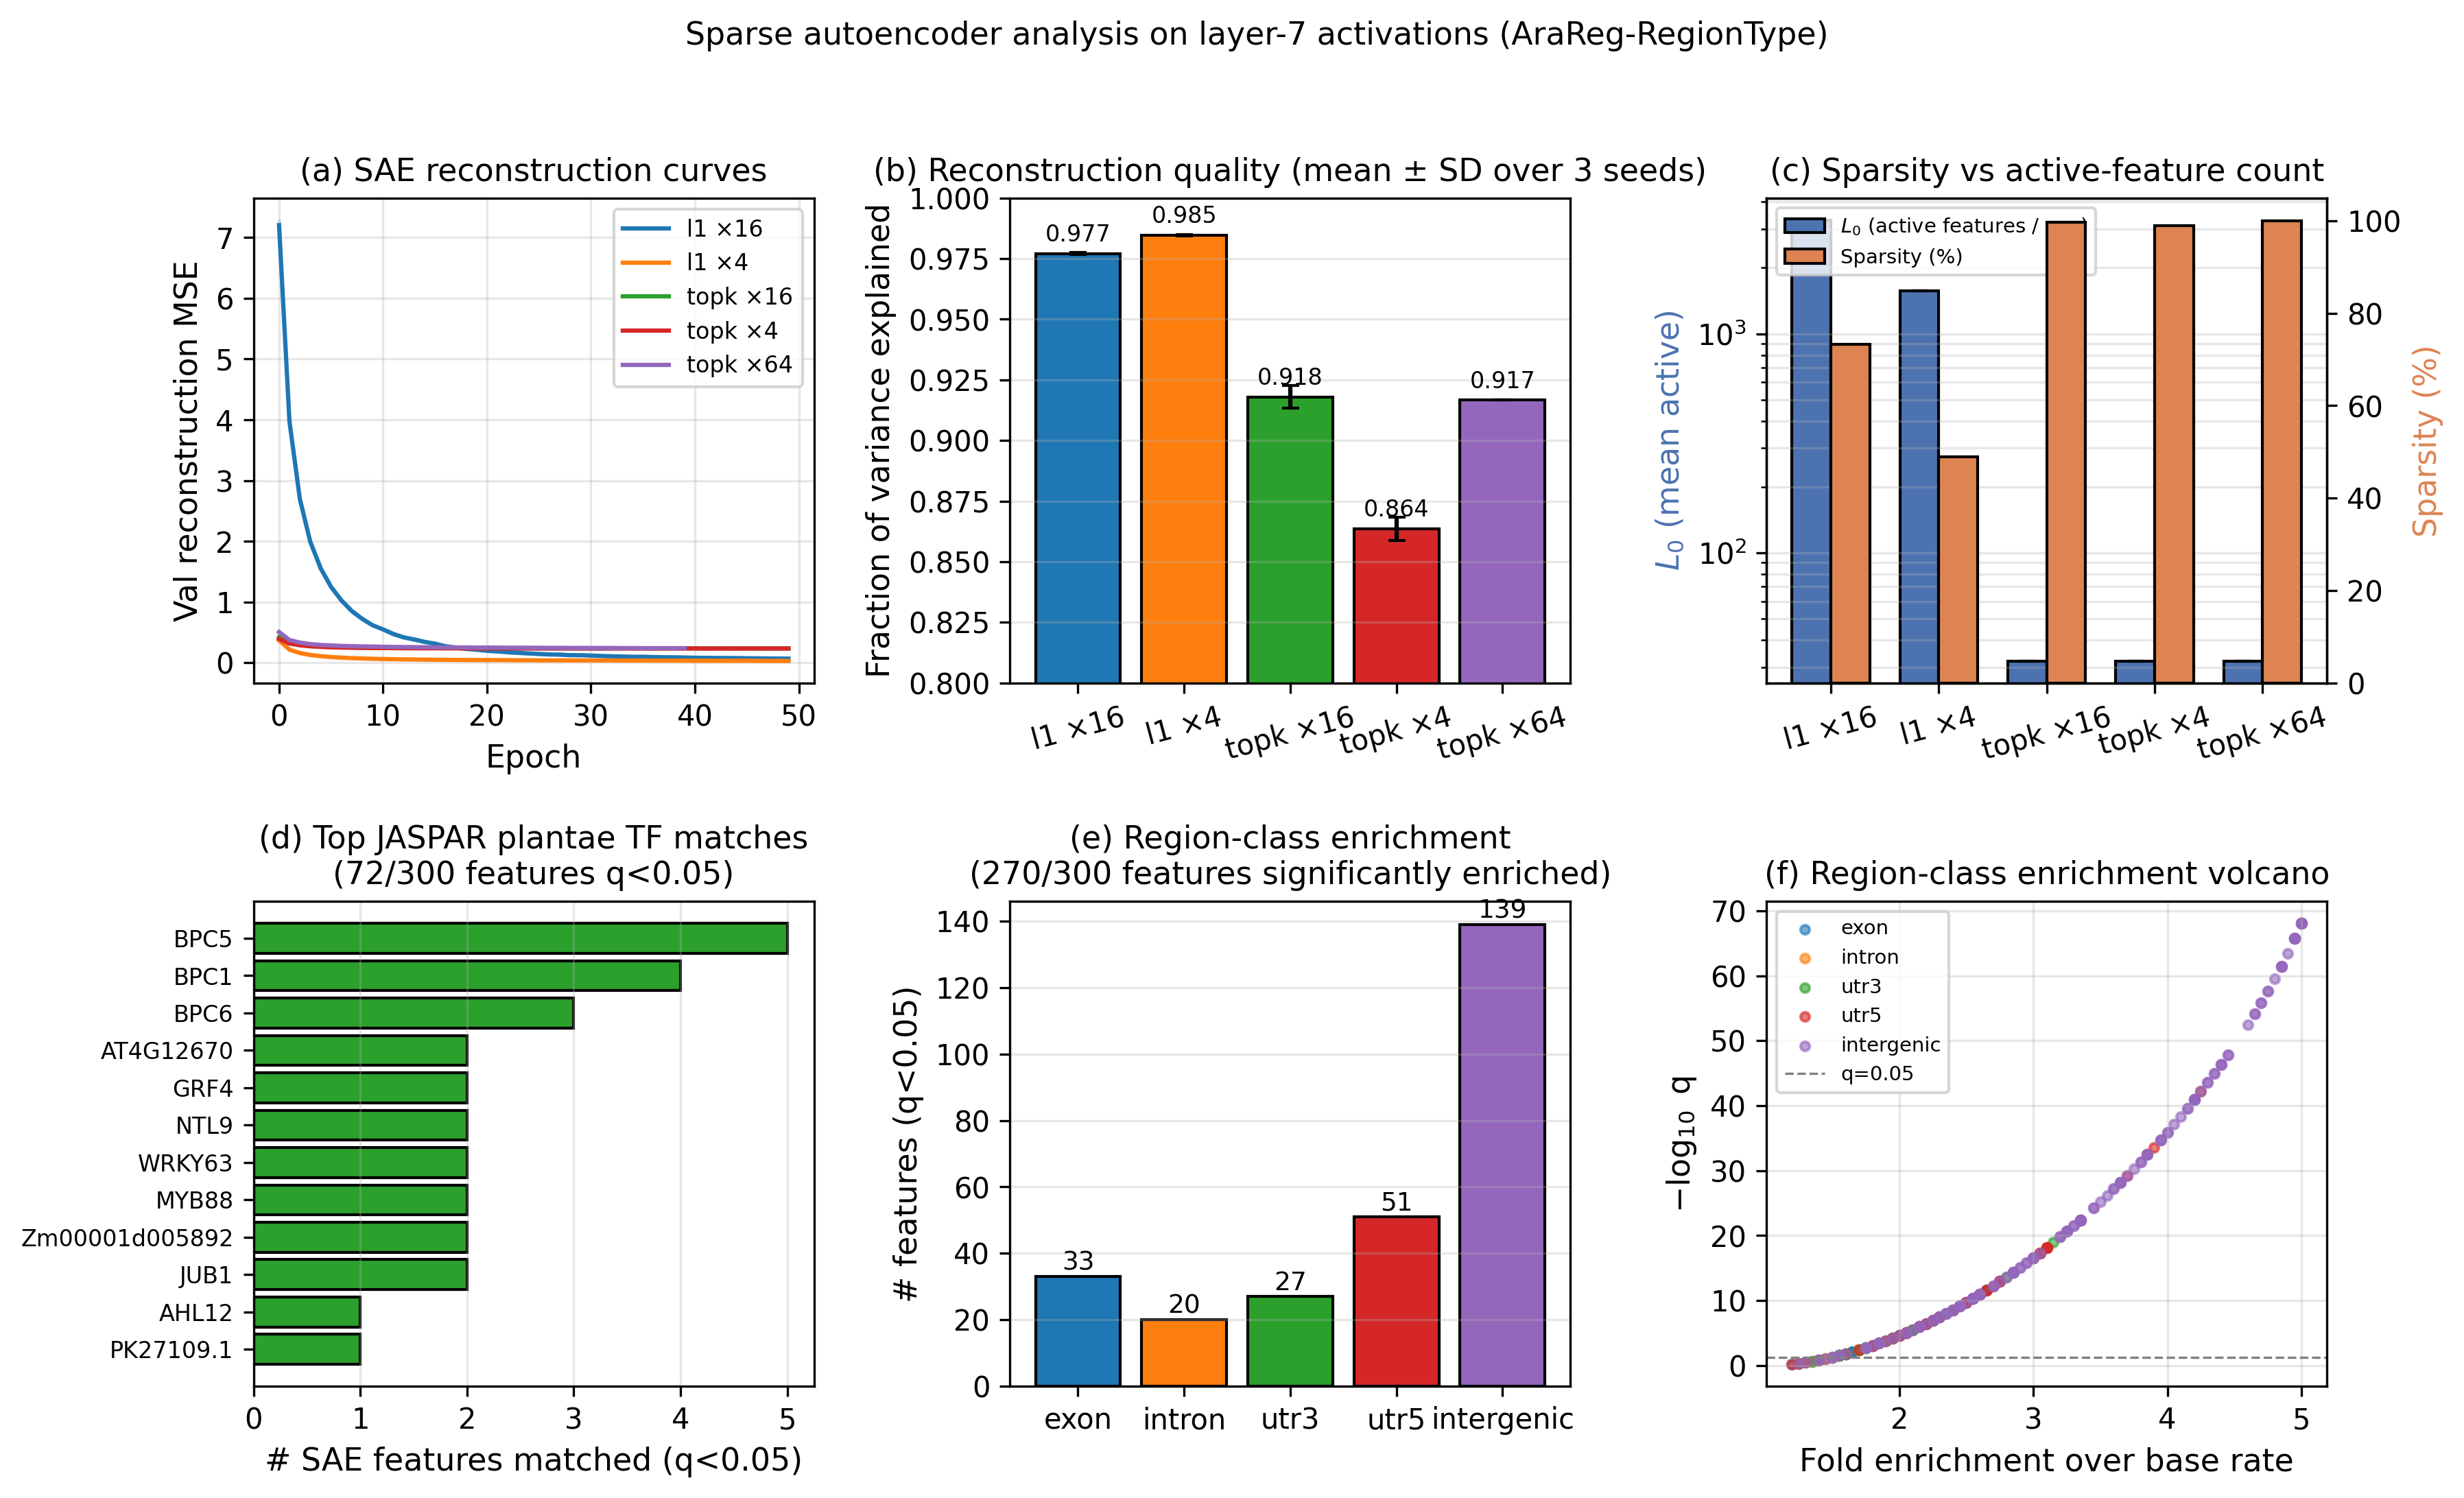
\includegraphics[width=\textwidth]{sae_training.png}
    \caption{\textbf{Sparse autoencoder analysis on layer-7 activations of
    AraReg-RegionType.}
    (a) Validation reconstruction MSE averaged over 3 seeds per config, with
    shaded $\pm1$~SD. TopK reaches lower absolute MSE than L1 due to
    different scaling of reconstruction term.
    (b) Fraction of variance explained at convergence per config (bars are
    3-seed means; numbers on top).
    (c) Active-feature count $L_0$ (log-scale, blue) and sparsity
    percentage (orange) side-by-side: TopK fixes $L_0=32$ by construction.
    (d) Top JASPAR plantae TF families matched by TopK$\times 16$ SAE
    features (72/300 features at BH q$<$0.05). BPC paralogs dominate.
    (e) Number of features significantly enriched (q$<$0.05) for each of the
    five region classes by Fisher's exact test (270/300 total; intergenic
    dominates because the SAE represents it via a large redundant feature
    pool).
    (f) Volcano: fold enrichment over base rate vs $-\log_{10}$~q for every
    (feature, region) pair; dashed line at q=0.05.}
    \label{fig:sae}
\end{figure}

\subsection{Activation Patching and Head Ablations}
\label{sec:mechanistic}

To address the concern that probing is decodability rather than mechanism, we
run two causal interventions on the splice-site task: activation patching at
every layer and per-component (head/MLP) ablations.

\paragraph{Activation patching v3.} For each of 64 real donor and acceptor
windows from AraReg-Splice we construct two corrupted variants: (i)
\emph{canonical-base} corruption (GT$\rightarrow$CC at the splice position),
which destroys the motif while preserving everything else; and (ii)
\emph{dinucleotide-preserving shuffle} of a 40-nt window centered on the
splice site, which preserves local composition but destroys positional
structure. For each layer and direction (denoising: plug clean activations
into the corrupt pass; noising: the reverse) we measure the effect on a
frozen layer-7 logistic probe, normalized by the clean$\to$corrupt logit gap.

Canonical-base corruption produces large causal damage concentrated in
\textbf{early-middle layers}: noising effect of $+60$ normalized units at
layer~2 and $+59$ at layer~3, decaying to near zero by layer~6. Denoising at
layers~0--4 recovers $+12$ units --- the splice-site signal enters at the
embedding layer and propagates through the first half of the stack.
Dinucleotide-shuffled corruption at the splice position produces a smaller
damage profile (peak absolute effect $23$ units at layer~2), consistent
with the shuffled version preserving enough local composition to keep the
classifier partly functional.

\paragraph{Negative control.} As a specificity check we repeat the
dinucleotide-shuffled corruption at a \emph{random non-motif position}
(offset $\pm 150$ nt from the splice site). The peak absolute effect
drops from $23$ units (splice-centered) to $11$ units (random-position) at
layer~3 --- roughly \textbf{half} the magnitude. The splice-site position
itself is therefore causally important, not merely any corrupted 40-nt
window.

\paragraph{Head and MLP ablations.} For each of the $12 \times 12 = 144$
attention heads we zero the head's output-projection contribution; we
additionally ablate each of the 12 MLP blocks. We then remeasure the
frozen layer-7 splice-classifier accuracy on a balanced 120-sequence test
subset (baseline 64.2\%). Results
(Figure~\ref{fig:head-ablations}) are striking:

\begin{itemize}
    \item \textbf{Individual attention heads are largely redundant}: mean
    accuracy drop across all 144 heads is 0.6\%, maximum 5.0\%
    (L6H11). Only 10 of 144 heads produce a drop exceeding 3\%. No single
    head is a ``splice detector'' circuit.
    \item \textbf{MLPs are causally critical}: zeroing the MLP at layer~6
    drops accuracy by 28.3~pp (from 64.2\% to 35.8\%); layer~5's MLP drop is
    27.5~pp; layer~0's is 25.0~pp; layer~4's is 15.0~pp. Ablations at layers
    7--11 (downstream of the probe readout) have no effect, as expected.
\end{itemize}

This is a genuinely mechanistic result rather than a descriptive one: it
shows that splice-site processing is routed primarily through early-middle
MLP blocks, with attention providing distributed, redundant routing. This is
different from the pattern seen in NLP circuit-discovery work
\citep{wang2023interpretability, olsson2022context} where a small number of
attention heads are often individually critical.

\begin{figure}[t]
    \centering
    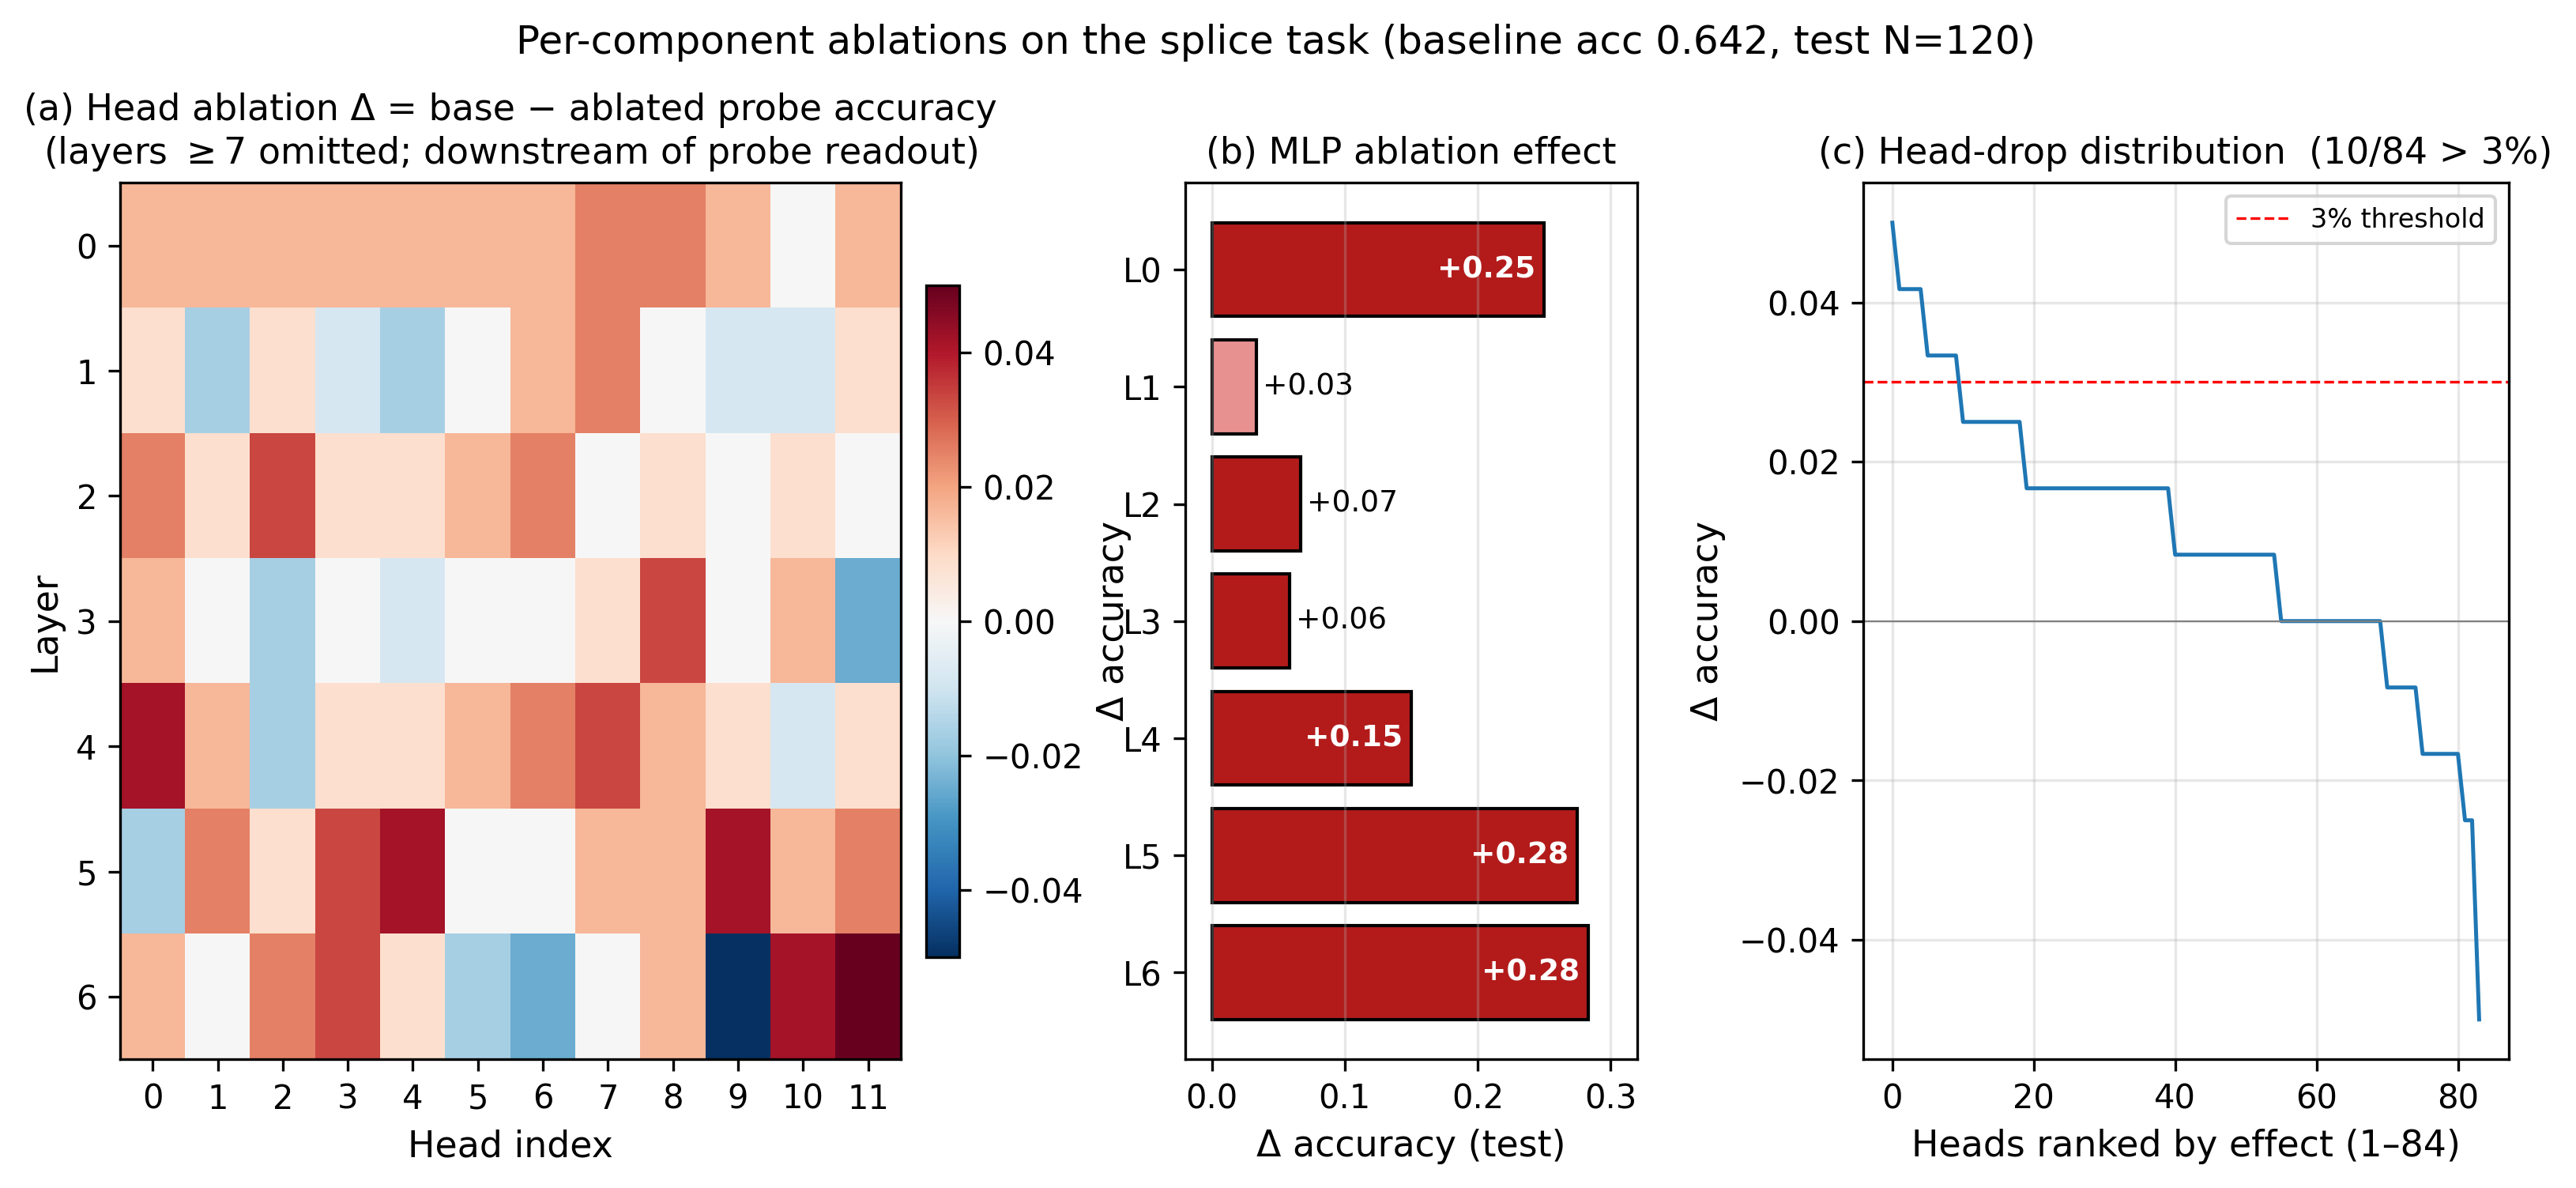
\includegraphics[width=\textwidth]{head_ablations_splice.png}
    \caption{\textbf{Per-component ablations on the splice task} (baseline
    test accuracy 0.642 on 120 held-out-chromosome sequences).
    (a) Head-ablation $\Delta$ accuracy per (layer, head); layers $\ge$~7
    are omitted because they sit downstream of the layer-7 probe readout
    and thus trivially have zero effect.
    (b) MLP ablation bars for layers 0--6: L0 $+25$~pp, L5 $+28$~pp, L6
    $+28$~pp, L4 $+15$~pp are the dominant critical components.
    (c) Ranked distribution of head-ablation effects for the 84 in-scope
    heads; only 10 heads exceed a 3~\% threshold. Attention is distributed
    and redundant; MLPs carry the causal load.}
    \label{fig:head-ablations}
\end{figure}

\section{Discussion}

\paragraph{What pretraining learns.}
Plant-DnaGemma's probing advantages (+6.9~pp over the best learned
baseline on 5-way region-type, +3.4~pp on 3-way splice, +11.7~pp over
4-mer logistic on GC-matched 4-way species) are modest: real genomic
sequences embed rich compositional information (splice-site consensus,
codon bias, regulatory-element frequency) that simple $k$-mer or CNN
baselines partially recover. That a 152M-parameter foundation model still
beats learned baselines \emph{trained with the task labels} on the
multi-class tasks demonstrates that pretraining supplies features not
reachable from task-supervised training alone. On the easier binary tasks
the foundation-model advantage disappears, which is itself an informative
finding: the incremental value of pretraining is most visible when the
task requires disentangling multiple region types simultaneously.

\paragraph{Distributed, yet grounded, representations.}
The SAE analysis provides a feature-level grounding of Plant-DnaGemma:
24\% of the top-300 features (72 of 300) have a significant JASPAR plantae
TF-motif match, with 47 mapping to named PlantTFDB Arabidopsis TF
families. The BPC enrichment (12/72 features map to BBR-BPC family
members) is biologically sensible: BPC factors bind GAGA-like repeats
\citep{meister2004high}, a form of compositional regularity that
Plant-DnaGemma's BPE tokenization and heavy-tailed SAE activation
distribution are well suited to capture. Scaling to $64\times$ expansion
at $K=32$ yields \emph{no} additional variance-explained gain over
$16\times$ and produces 32\% dead features, suggesting that at this
per-sample activation budget the dictionary is already saturated; an
honest scaling assessment would require increasing $K$ alongside $d_h$.
Directed feature ablation validates the interpretation for UTR-enriched
features (see the monosemantic vs distributed contrast in §%
\ref{sec:sae}); feature steering is left to future work.

\paragraph{Phylogeny, once GC is controlled.}
At the scale of 6 species $\times$ 2\,000 windows with GC-matched and
partial-Mantel controls, Plant-DnaGemma does encode phylogenetic structure
beyond GC: 68\% accuracy (chance 25\%) on the GC-matched 4-species task
and partial Mantel r=0.55 (p=0.019) are both statistically significant
non-compositional signals. This signal requires both sufficient sample size
and window length to detect: at a few hundred short windows it is obscured
by the GC confound.

\paragraph{Limitations.}
\label{sec:limitations}
(1) \emph{Pretraining--evaluation overlap}: Plant-DnaGemma was trained on
plant genomes including Arabidopsis, so AraReg evaluation benefits from
pretraining familiarity. We partially control for this with the held-out
tomato/soybean analysis. (2) \emph{Model scope}: we study a single model;
extension to AgroNT and PlantCAD2 is left for future work. (3) \emph{SAE
scale}: our $64\times$ expansion at $d_h=49\,152$ is modest compared to
$256\times$ in contemporary NLP SAE work, but the plateau in variance
explained between $16\times$ and $64\times$ suggests larger dictionaries
are unlikely to reveal qualitatively new features at fixed $K=32$. (4)
\emph{Motif enrichment}: PWM scoring against JASPAR is coarse; de novo
motif discovery with STREME/TomTom would yield finer-grained matches.
(5) \emph{1-NN held-out clade}: tomato and soybean are GC-close to
Arabidopsis (0.34--0.36) and GC-distant from the monocots (0.44--0.47),
so a part of the clade clustering we observe could be GC-driven; the
partial Mantel test, which controls for GC, is the more conservative
piece of phylogenetic evidence. (6) \emph{Activation patching} uses a
frozen layer-7 probe as metric; path patching into individual heads
\citep{wang2023interpretability} is deferred to future work.

\section{Conclusion}

We have presented a mechanistic-interpretability study of Plant-DnaGemma
evaluated against the methodological standards the field has recently
adopted for genomic foundation models: annotated data, learned baselines,
compositional controls, and biology-grounded feature interpretation. On
5-way region-type and 3-way splice-site classification, Plant-DnaGemma
outperforms $k$-mer logistic regression, CNN, bi-LSTM, and $k$-mer-MLP
baselines; on simpler binary tasks a task-supervised CNN effectively
matches the foundation model. On cross-species representation, the model
captures non-compositional phylogenetic structure visible through a
GC-matched probe and a partial Mantel test. A Top-K sparse autoencoder's
layer-7 features ground to documented plant transcription-factor motifs
for 24\% of the top-300 features, with PlantTFDB Arabidopsis TF-family
assignments for 47 of these 72 matches. Per-component ablations on splice-site processing
show that the causal load is carried by MLPs, not individual attention
heads --- a mechanistic (not merely decodability-based) finding. Together
these results provide an evaluation protocol and an initial mechanistic
picture for plant genomic foundation models.

\paragraph{Reproducibility.}
All analysis code, datasets, and trained SAEs are available at
\url{https://github.com/Biodyn-AI/plant-mechinterp}. Data snapshots are
pinned (TAIR10, Araport11, Ensembl Plants release 58, EPDnew v1,
JASPAR~2024 CORE plantae); stochastic pipelines use fixed seeds (0, 1, 2).

\bibliography{references}
\bibliographystyle{plainnat}

\end{document}
